% \documentclass[%
%  reprint,
%  amsmath,amssymb,
%  aps,
% ]{revtex4-2}
\documentclass[%
 reprint,
 amsmath,amssymb,
 aps,
]{revtex4-2}

\usepackage{float}

\usepackage{graphicx}% Include figure files
\usepackage{dcolumn}% Align table columns on decimal point
\usepackage{bm}% bold math
\usepackage{physics}
\setlength{\parskip}{\baselineskip}%
\usepackage{siunitx}
\usepackage[inline]{asymptote}
\usepackage{multirow}
\usepackage{tikz}
\usepackage{pgfplots, pgfplotstable}
\def\bibsection{\section*{\refname}} 

\usepackage{natbib}
\bibliographystyle{unsrtnat}

\pgfplotsset{compat=1.3}
\begin{document}

% \preprint{APS}

\title{Determining Uncertainties in the Free Fall Kinematics of a Dropping Paper}% Force line breaks with \\

\author{QiLin Xue}

\date{\today}% It is always \today, today,
             %  but any date may be explicitly specified

\begin{abstract}
This experiment determined the time it takes for a piece of paper to fall a distance of one meter and analyze how perturbations due to air resistance and initial conditions affects the distribution of times. It was found over $40$ trials that the average time was $1.25 \pm 0.01 \si{\second}$ with a standard deviation of $\sigma=0.06\si{\second}$. These results differ from the estimated maximum time of $1.2\si{\second}$, which shows that the effects of drag and lift were greater than what was expected.
\end{abstract}

%\keywords{Suggested keywords}%Use showkeys class option if keyword
                              %display desired
\maketitle

%\tableofcontents
\section{Introduction and Method}
For an object falling without the presence of air resistance, it experiences a constant acceleration $g$ and if it is dropped from rest, then the height it travels after a time $t$ is given by
\begin{equation}
    h=\frac{1}{2}gt^2
    \label{eq:}
\end{equation}
However, in the presence of air resistance, the acceleration becomes nonlinear. The resistive force of ar friction slows down the paper, increasing the time it takes to fall. I can estimate the magnitude of this force by considering the change in momentum of air molecules colliding with the paper. In a time $\dd{t}$, a mass of $\rho A \dd{x}$ collides inelastically with the paper. If the paper is moving at a speed $v$, then I can use Newton's second law to write the force of drag as:
\begin{equation}
    F_d \approx \frac{dp}{dt}=\frac{dm}{dt}v=\rho Av^2
    \label{eq:drag force}
\end{equation}
where I are ignoring edge effects. Here, $\rho$ is the density of air. The terminal velocity of the paper is given when the air friction balances out the gravitational force at the terminal velocity:
\begin{equation}
    v_T = \sqrt{\frac{\sigma g}{\rho}}
    \label{eq:terminal speed}
\end{equation}
where $\sigma \equiv \frac{m}{A}$ gives the area mass density of the paper. This places an upper limit of:
\begin{equation}
    t_\text{upper} = H\sqrt{\frac{\rho}{\sigma g}}
    \label{eq:}
\end{equation}
Paper with a density of $90 \si{\gram\per\square\meter}$ was used in this experiment over a distance of one metre. If the density of air takes on a typical value of $1.23 \si{\kilo\gram\per\metre\cubed}$\cite{ISA}, then the upper limit should be expected to be around $1.2\si{\second}$. However, since it is unrealistic to assume the paper will be parallel to the ground at all times, the average drag force will be lower and thus I predict there will be numerous results below this upper bound.

To minimize uncertainties in the initial height the paper was dropped from as well as the initial angle, three strings were tied from the ceiling and a metre stick was used to measure the tips to be $1 \text{ m}$ above the floor. The three strings define a horizontal plane such that if a piece of paper lightly touches all three ends, then it is safely at a horizontal position with respect to the ground. To a precision of $\pm 0.5 \si{\milli\meter}$, the meter stick was used to measure the height of the tip from the ground. The bottom was placed flat on the ground to minimize angle uncertainties.

The drops were recorded using a $29.97\text{ fps}$ High Definition 1080p camera and the time elapsed between when the paper gets released and when it first touches the ground was determined by playing the video frame by frame in a video player afterwards. Markings were also made on the ground at the location where each paper initially made contact to analyze uncertainties in the initial orientation. The paper was always held in the same orientation with the long end facing the camera.

\section{Results}
A total of $40$ trials were completed with an average of $1.25\si{\second}$ such that the time uncertainty is related to the time of $1$ frame or $1/29.97^\text{th}$ of a second. The measurement uncertainty for each measurement is estimated to be $\pm 0.01 \si{\second}$, which is $40\%$ of the time of a single frame. The specific ratio of $1/3$ is justified in the discussion. This is smaller than the standard deviation of the data set: $\sigma_\text{deviation}=0.06\si{\second}$.
\begin{figure}[!h]
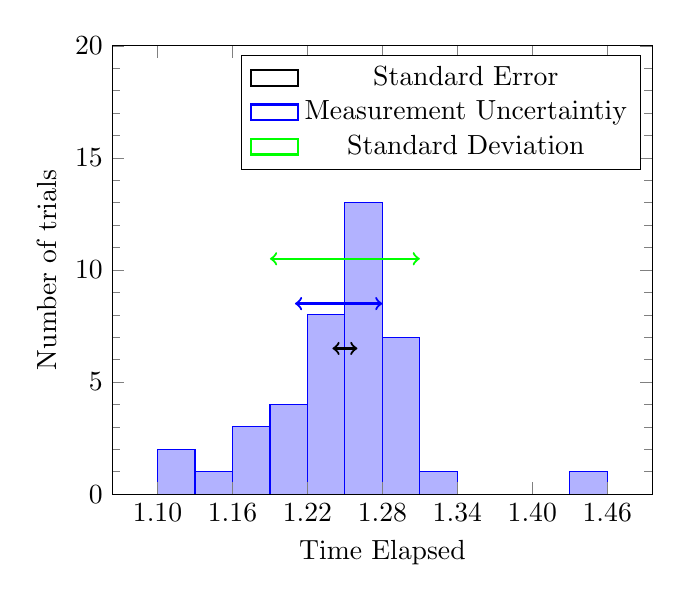
\begin{tikzpicture}
    \begin{axis}[
        ymin=0, ymax=20,
        xtick={1.1,1.16,...,1.46},
        xticklabels={$1.10$, $1.16$, $1.22$,  $1.28$, $1.34$,$1.40$,$1.46$},
        minor y tick num = 4,
        area style,
        ylabel={Number of trials},
        xlabel={Time Elapsed},
        % x tick label style={rotate=-45}
        ]
    \addplot+[ybar interval,mark=no,forget plot] plot coordinates { (1.10, 2) (1.13,1) (1.16,3) (1.19,4) (1.22, 8) (1.25, 13) (1.28, 7) (1.31,1) (1.34,0)(1.37,0)(1.40,0)(1.43,1)(1.46,0)};

    \addplot[black,sharp plot,thick,<->]
    coordinates {(1.24,6.5) (1.26,6.5)}
    ;
    \addlegendentry{Standard Error}

    \addplot[blue,sharp plot,thick,<->]
    coordinates {(1.21,8.5) (1.28,8.5)}
    ;
    \addlegendentry{Measurement Uncertaintiy}

    \addplot[green,sharp plot,thick,<->]
    coordinates {(1.19,10.5) (1.31,10.5)}
    ;
    \addlegendentry{Standard Deviation}
    \end{axis}
    \end{tikzpicture}
    \caption{Distribution of times in the experiment. The standard deviation, measurement uncertainty, and standard error are shown.}
    \label{fig:histogram}
\end{figure}
The distribution can be seen in the histogram in figure \ref{fig:histogram}. The bin width was chosen to be half the standard deviation such that in each bin, there are few statistical outliers which may give an inaccurate picture of the distribution, but there were enough bins to show the skewed pattern. The median time (which is also the mode) was $1.27 \si{\second}$, which is half a standard deviation higher than the average. This supports the initial hypothesis of negatively skewed data. However, the upper bound was measured to be around $1.33\pm 0.05\si{\second}$, which was slightly higher than the predicted value.

Since the statistical uncertainty for each measurement is higher than the measurement uncertainty, I estimate two thirds of all measurements will fall in the range of:
\begin{equation}
    t = 1.25 \pm 0.06 \si{\second}
    \label{eq:}
\end{equation}
The standard error on the other hand is $\sigma_\text{error} = 0.01\si{\second}$, and coincidentally the measurement error is also the same, though it is slightly bigger. As a result, two thirds of all averages taken over $40$ trials would fall in the range of:
\begin{equation}
    t_\text{avg} = 1.25 \pm 0.01 \si{\second}
    \label{eq:}
\end{equation}
Justification is provided in the discussion and technical details is given in Appendix A. When the uncertainty and standard error are graphed against the number of trials in figure \ref{graph:line chart}, I see that there is no noticeable trend to the standard deviation, but there is a noticeable downwards trend to the standard error. The error bars eventually cross the $x$ axis, which show that $\sigma/\sqrt{N}$ is not a reliable measure of the uncertainty of the average and the measurement uncertainty has to be used instead.
\begin{figure}[!h]
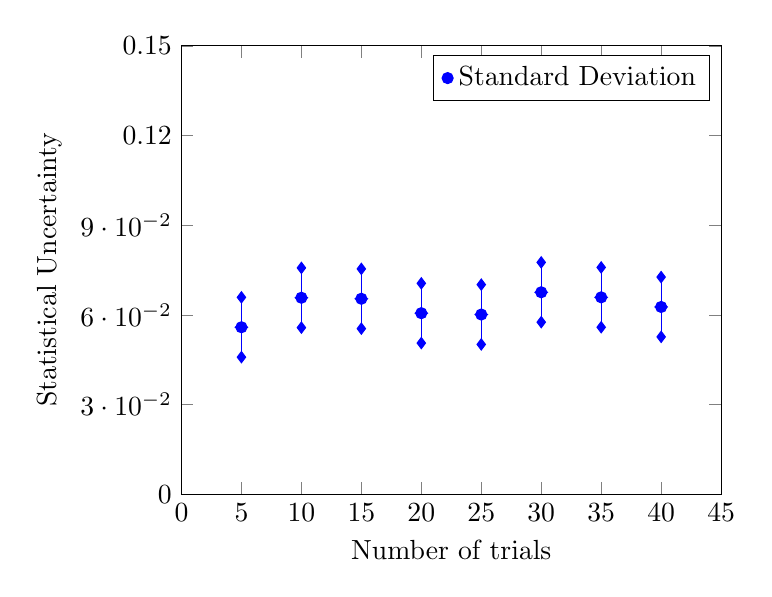
\begin{tikzpicture}
    \begin{axis}[
        xlabel=$x$,
        ylabel=$y$,
        xmin=0, xmax=45,
        ymin=0, ymax=0.15,
        xtick={0,5,...,45},
        ytick={0,0.03,...,0.15},
        xlabel={Number of trials},
        ylabel={Statistical Uncertainty},
    ]
    
    % Standard Deviation
    \addplot[color=blue,mark=*,only marks,error bars/.cd,
    y dir=both,y explicit,
    x dir=both,x fixed=0.05,
    error mark=diamond*] coordinates {
        (5,0.05583316827) +-  (0,0.01)
        (10,0.06570595256) +- (0,0.01)
        (15,0.06536889303) +- (0,0.01)
        (20,0.06054107296) +- (0,0.01)
        (25,0.06009094721) +- (0,0.01)
        (30,0.06753400077) +- (0,0.01)
        (35,0.06584424028) +- (0,0.01)
        (40,0.06262313515) +- (0,0.01)
    };
    \addlegendentry{Standard Deviation}
    
    \end{axis}
        \end{tikzpicture}
        \pgfplotsset{scaled y ticks=false}

        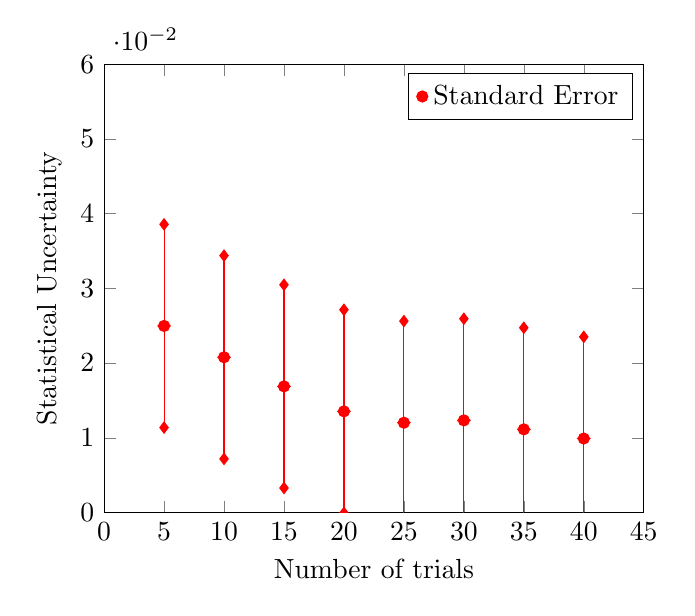
\begin{tikzpicture}
    \begin{axis}[
        xlabel=$x$,
        ylabel=$y$,
        xmin=0, xmax=45,
        ymin=0, ymax=0.06,
        xtick={0,5,...,45},
        ytick={0,0.01,...,0.06},
        xlabel={Number of trials},
        ylabel={Statistical Uncertainty},
    ]
    
    \addlegendentry{Standard Error}
    
    \addplot[color=red,mark=*,only marks,error bars/.cd,
    y dir=both,y explicit,
    x dir=both,x fixed=0.05,
    error mark=diamond*]
        coordinates {
            (5,0.02496935193) +- (0,0.0136)
            (10,0.02077804659) +- (0,0.0136)
            (15,0.0168781756) +- (0,0.0136)
            (20,0.01353739546) +- (0,0.0136)
            (25,0.01201818944) +- (0,0.0136)
            (30,0.01232996521) +- (0,0.0136)
            (35,0.01112970796) +- (0,0.0136)
            (40,0.009901587065) +- (0,0.0136)
        };
    % \addplot[color=red,mark=*,error bars/.cd,
    % y dir=both,y explicit,
    % x dir=both,x fixed=0.05,
    % error mark=diamond*]
    %     coordinates {
    %         (5,0.02496935193) +- (0,0.02)
    %         (10,0.02077804659) +- (0,0.02)
    %         (15,0.02) +- (0,0.008520563362)
    %         (20,0.02) +- (0,0.007379024326)
    %         (25,0.02) +- (0,0.0066)
    %         (30,0.02) +- (0,0.006024948133)
    %         (35,0.02) +- (0,0.005578018081)
    %         (40,0.02) +- (0,0.005217758139)
    %     };
    \addlegendentry{Standard Error}
    \end{axis}
        \end{tikzpicture}
        \caption{The standard error and the standard deviation plotted against the number of trials, in multiples of five. The measurement uncertainty is also shown via error bars.}
        \label{graph:line chart}
    \end{figure}
The spatial distribution of the contact points can be seen in figure \ref{fig:scatter}. While most contact points are relatively near the triangle, it is biased towards the top and towards the right. 
\begin{figure}[!h]
    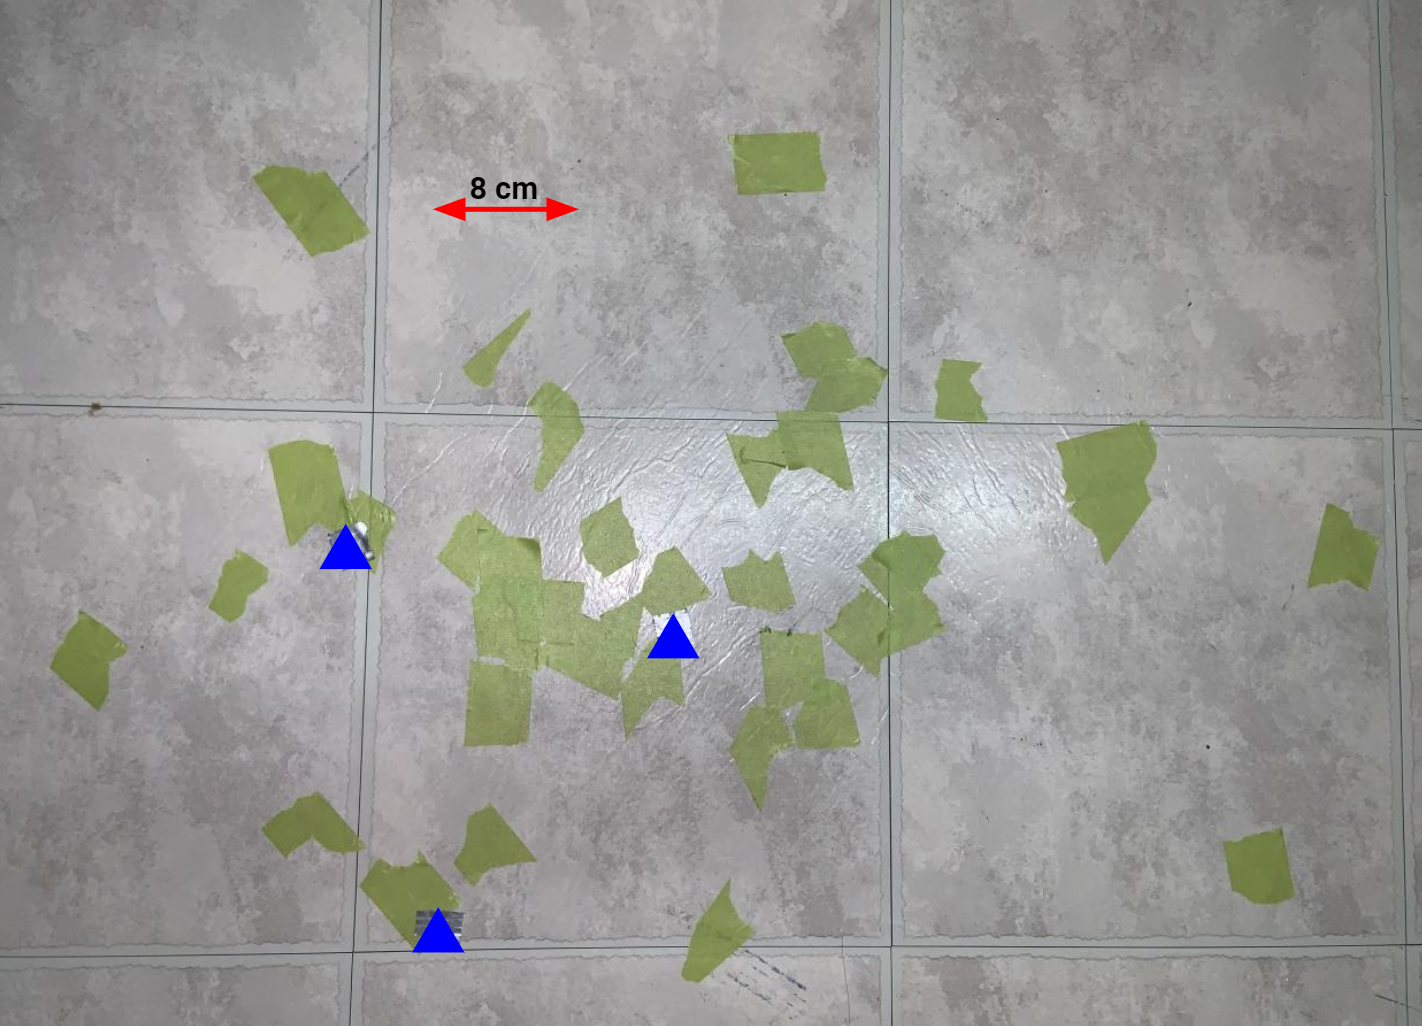
\includegraphics[width=\linewidth]{scatter.png}
    \caption{Map of points of contact with the ground. The location of the three strings are denoted by the blue triangles and the contact point of each drop is recorded with green tape. The length of the red line is $8\si{\centi\metre}$. The paper was held parallel to the tile markings.}
    \label{fig:scatter}
\end{figure}
\section{Discussion}
\subsection{Measurement Uncertainties}
I have made the claim that the largest measurement uncertainties were due to the limited frame rate of the recording device. In this section, other sources of uncertainty will be explored and show they are below $\Delta t = 0.05 \si{\second}$.

I estimate the uncertainty of the initial height to be around $\Delta h \approx 1 \si{\milli\meter}$. As I shall show, this uncertainty isn't significant at all and any fluctuations would be negligible. I was able to make readings on the meter stick with an accuracy of $\pm 0.5 \si{\milli\meter}$, but I estimate my shaky hands to have an additional uncertainty of $\pm 0.5 \si{\milli\meter}$. This small uncertainty is due to the setup: Since I have strings tied from the top, it stops me from bringing the paper too high or too low. Extra time was sacrificed in order to line the paper up accurately. Making the assumption that the paper reaches terminal velocity very quickly, the time elapsed is proportional to the height of the fall, so the time uncertainty as a result of this is:
\begin{equation}
    \Delta t_\text{from height} = t\frac{\Delta h}{h} \approx 0.001 \si{\second}
    \label{eq:}
\end{equation}
There can also be uncertainty in the initial angle the paper is held at. I make the assumption that the horizontal displacements shown in figure \ref{fig:scatter} correspond to a nonzero initial angle. As an approximate estimation, I can designate each trial that lands outside the central square region as a trial where the angle wasn't controlled well. I then determine the average of these trials to be $t_\text{far}=1.26 \pm 0.02\si{\second}$. On the other hand, the average time for trials that landed in the central region was $t_\text{central}=1.24 \pm 0.01 \si{\second}$. On average, only $14/40=35\%$ of papers went outside the region so I estimate that the time uncertainty that is a result of uneven hands is thus:
\begin{equation}
    \Delta t_\text{from angle} \approx 35\% \cdot 0.02\si{\second} = 0.007 \si{\second}
    \label{eq:angle uncertainty}
\end{equation}
Note that the initial speed also has an uncertainty, as it is unrealistic to drop an object perfectly at rest using hands. This uncertainty however can fall under both the uncertainty of the height and the uncertainty of the initial angle. In order to match the uncertainty of the frames, I would have needed to toss the paper up a distance of $30\si{\milli\meter}$, which could not have been possible due to the strings blocking the motion. There also could not be an initial downwards velocity since I let go of my top fingers before my bottom fingers so there cannot be any pushing force downwards.

Similarly, if there was instead some initial horizontal velocity, then the discussion above involving trials where the paper traveled far from the drop location would have also covered it.

All three of these uncertainties are smaller than the uncertainties used in the observations section, so ignoring them can be justified for the sake of simplicity. There are other uncertainties as well, such as the paper being crinkly and tiny wind currents causing perturbations were not able to be quantified, and are classified under statistical errors.

In figure \ref{graph:line chart}, I made the claim that the measurement uncertainties were independent of one another. This is justified by how I determined the elapsed time. I let my starting frame be the first frame where I can see that the paper was not in contact with my fingers. The final frame was thus the first frame where I saw the paper make contact with the ground. The time was determined by counting the frames and dividing it by the frames per second ($\text{fps}$). Let $0<\delta t < 1/\text{fps}$, then the actual time of the initial drop is $t_1-\delta t_1$ and the actual time of when the paper makes contact is $t_2-\delta t_2$. If $\delta t_2 > \delta t_1$, the actual elapsed time is shorter than the measured. If $\delta t_2 < \delta t_1$, the actual elapsed time is longer than measured. Since both of these will have equal probabilities of happening, it is just as likely for each value to be overestimated than underestimated.

Earlier, we claimed that the time measurement uncertainty for each trial is $40\%$ of a frame. Let $t_1$ and $t_2$ be random variables evenly distributed in the normalized range $[0,1]$ such that their difference gives the uncertainty in the time measurement, in units of the fps. The uncertainty is then given by:
\begin{equation}
    \sigma^2 = \langle (t_2-t_1)^2 \rangle - \langle t_2-t_1 \rangle^2
    \label{eq:}
\end{equation}
where $\langle t_2-t_1 \rangle$ represents the expected value of the difference. Due to the symmetry of the setup, the expected value of the difference is zero since it is just as likely to end up positive than negative. The expected value of the square of the difference is given by:
\begin{equation}
    \langle (t_2-t_1)^2 \rangle = \int_0^1\int_0^1 (t_2-t_1)^2 \dd{t_2}\dd{t_1} = \frac{1}{6}
    \label{eq:}
\end{equation}
Therefore:
\begin{equation}
    \sigma = \frac{1}{\sqrt{6}} \approx 0.41
    \label{eq:}
\end{equation}
of a frame, or $\sigma=0.014 \approx 0.01\si{\second}$. Another important feature of figure \ref{graph:line chart} is that the average measurement uncertainties do not change. This is because the time uncertainty is evenly distributed and does not follow a normal distribution.

\subsection{Lift Phenomenon}
From the previous section, it was discovered that papers which traveled farther also traveled longer. This contradicted the hypothesis, which assumed there was a hard upper bound, and that papers which don't fall perpendicular will spend less time in the air.

Qualitative observations show otherwise. In many trials where papers flew down, they were able to angle up and coast at a constant altitude before touching the floor, reminding me of a bird extending its wings at the last second of a dive. Other times, it rocked back and forth. In both these scenarios, the flexible nature of the paper was able to generate lift, which causes the paper to stay in the air longer than theoretical estimates.

\section{Conclusion}
The purpose of the lab was to determine three numbers $X$, $Y$, and $Z$ such that if this experiment was to be reproduced, two thirds of data points would fall in the range of $X\pm Y$, and if this experiment was done numerous times, the average would fall in the range of $X \pm Z$ two thirds of the time.

These numbers were determined to be \begin{align*} 
    X=1.25 \si{\second} \\
    Y=0.06\si{\second} \\ 
    Z=0.01\si{\second}
\end{align*}
To improve this experiment, a better camera with a higher frame rate can be used to lower the time uncertainty of the drop. Human error can be avoided by designing a mechanical device that can hold the paper still at a specific height and drop it instantaneously on command, though this second improvement should not be prioritized on.

These changes will reduce measurement and systemic errors, and in turn, also lower the standard deviation, allowing a deeper look into the chaotic motion of the paper as it falls down.

\onecolumngrid

\bibliography{citations}

\newpage
\appendix

\section{Justification for $Y$ and $Z$ values.}
To be clear, $Y$ represents the standard deviation in this experiment. If the distribution is assumed to be normally distributed, then around 68\% of data points will fall within $X-Y$ and $X+Y$ where $X$ is the mean. Technically, a more formal approach would involve z-scores. However, due to the high uncertainties in the other variables, the difference would be negligible.

The standard error gives the statistical uncertainty of an average. Intuitively, this uncertainty should go down with an increased number of trials. This is shown in figure \ref{graph:line chart}. The standard deviation however, stays constant, so it is a better measure of the statistical uncertainty of a single datum, further justifying why $Y$ is the standard deviation.

A proof for why the standard error is exactly $\frac{\sigma}{\sqrt{N}}$ is provided below. Suppose that the data is normally distributed, which allows us to add in quadrature:
\begin{equation}
    \sigma(t_\text{avg})^2=\sigma(t_1/N)^2+\sigma(t_2/N)^2+\cdots+\sigma(t_N/N)^2
    \label{eq:}
\end{equation}
Letting $\sigma(t_1) = \sigma(t_2) = \cdots = \sigma(t_N)$, this simplifies to:
\begin{equation}
    \sigma (t_\text{avg}) = \frac{\sigma (t)}{\sqrt{N}}
    \label{eq:}
\end{equation}
The value of $Z$ is chosen as the maximum between the measurement error and the standard error. The measurement error is larger by a tiny bit (from the discussion, I derived it to $\frac{1}{29.97\sqrt{6}}\approx 0.014 \si{\second}$, where I have included an extra significant digit). The standard error on the other hand, is: $\frac{\sigma}{\sqrt{40}}=0.0010$.
\section{Data Table}
\begin{table}[h!]
    \centering
    \begin{tabular}{|c|c|c|}
    \hline
    Trial & Frames & Seconds \\ \hline
    % 1 & $2.22 \pm 0.0098$ & $2.07 \pm 0.0082$ \\ \hline
    % 2 & $2.35 \pm 0.0088$ & $1.97 \pm 0.0096$ \\ \hline
    % 3 & $2.37 \pm 0.0069$ & $1.94 \pm 0.0045$ \\ \hline
    1	&37&	1.235 \\ \hline
    2	&33&	1.101 \\ \hline
    3	&35&	1.168 \\ \hline
    4	&33&	1.101 \\ \hline
    5	&35&	1.168 \\ \hline
    6	&38&	1.268 \\ \hline
    7	&39&	1.301 \\ \hline
    8	&36&	1.201 \\ \hline
    9	&36&	1.201 \\ \hline
    10	&37&	1.235 \\ \hline
    11	&38&	1.268 \\ \hline
    12	&38&	1.268 \\ \hline
    13	&39&	1.301 \\ \hline
    14	&35&	1.168 \\ \hline
    15	&38&	1.268 \\ \hline
    16	&38&	1.268 \\ \hline
    17	&38&	1.268 \\ \hline
    18	&38&	1.268 \\ \hline
    19	&38&	1.268 \\ \hline
    20	&38&	1.268 \\ \hline
    \end{tabular}
    \begin{tabular}{|c|c|c|}
        \hline
        Trial & Frames & Seconds \\ \hline
        21	&34&	1.134 \\ \hline
        22	&38&	1.268 \\ \hline
        23	&38&	1.268 \\ \hline
        24	&39&	1.301 \\ \hline
        25	&37&	1.235 \\ \hline
        26	&37&	1.235 \\ \hline
        27	&36&	1.201 \\ \hline
        28	&38&	1.268 \\ \hline
        29	&39&	1.301 \\ \hline
        30	&43&	1.435 \\ \hline
        31	&40&	1.335 \\ \hline
        32	&39&	1.301 \\ \hline
        33	&39&	1.301 \\ \hline
        34	&38&	1.268 \\ \hline
        35	&37&	1.235 \\ \hline
        36	&37&	1.235 \\ \hline
        37	&37&	1.235 \\ \hline
        38	&39&	1.301 \\ \hline
        39	&36&	1.201 \\ \hline
        40	&37&	1.235 \\ \hline
        \end{tabular}
    \caption{Data regarding the elapsed time was collected by counting frames in the video recording. The frames were manually converted to seconds by dividing by the frame rate of $29.97$ fps. An extra significant digit for intermediate calculation purposes, and the statistical uncertainty of each datum is $\pm 0.06 \si{\second}$}
    \end{table}
\end{document}
% %
% % ****** End of file apssamp.tex ******